\setcounter{section}{2}
\section{SIFT Keypoint Descriptor	}
Unter der Annahme, dass das Sampling relativ zur dominanten Richtung durchgeführt wurde,
ist der Keypoint Descriptor gegeben durch:
$$
	\begin{pmatrix}
		0    \\
		0.94 \\
		0.03 \\
		0.03 \\
		0    \\
		0    \\
		0    \\
		0    \\
		0    \\
		0.03 \\
		0.91 \\
		0    \\
		0    \\
		0.03 \\
		0.03 \\
		0    \\
	\end{pmatrix}
$$
\begin{figure}
	\centering
	\begin{subfigure}{\textwidth}
		\centering
		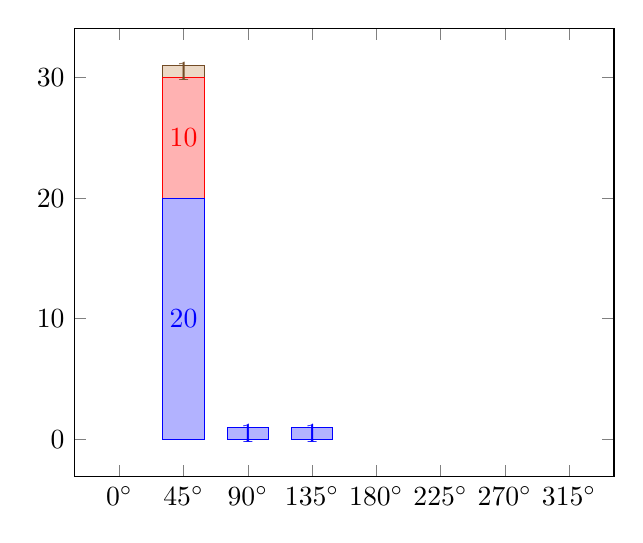
\begin{tikzpicture}
			\begin{axis}[
					ybar stacked,
					bar width=15pt,
					nodes near coords,
					symbolic x coords={bin1, bin2, bin3, bin4,
							bin5, bin6, bin7, bin8},
					xtick=data,
					xticklabels={$0^\circ$,
							$45^\circ$,
							$90^\circ$,
							$135^\circ$,
							$180^\circ$,
							$225^\circ$,
							$270^\circ$,
							$315^\circ$,
						}
				]
				\addplot+[ybar] plot coordinates {(bin1,0) (bin2,20) (bin3,1) (bin4,1) (bin5,0) (bin6,0) (bin7,0) (bin8,0)};
				\addplot+[ybar] plot coordinates {(bin1,0) (bin2,10) (bin3,0) (bin4,0) (bin5,0) (bin6,0) (bin7,0) (bin8,0)};
				\addplot+[ybar] plot coordinates {(bin1,0) (bin2,1) (bin3,0) (bin4,0) (bin5,0) (bin6,0) (bin7,0) (bin8,0)};
			\end{axis}
		\end{tikzpicture}
		\caption{Obere Teilregion}
	\end{subfigure}
	\par\bigskip
	\begin{subfigure}{\textwidth}
		\centering
		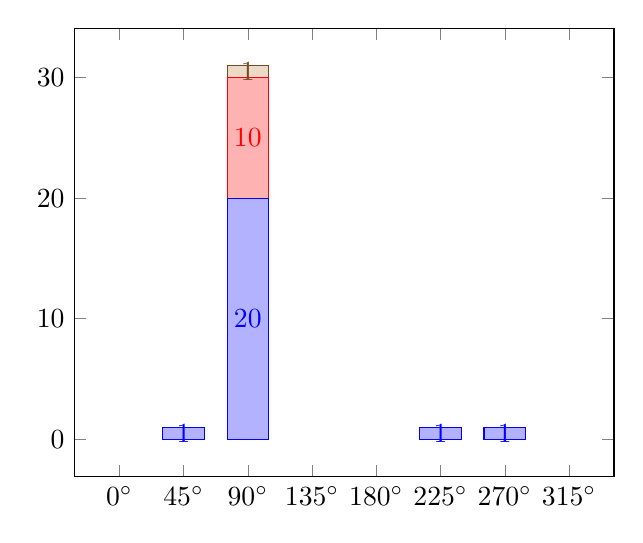
\begin{tikzpicture}
			\begin{axis}[
					ybar stacked,
					bar width=15pt,
					nodes near coords,
					symbolic x coords={bin1, bin2, bin3, bin4,
							bin5, bin6, bin7, bin8},
					xtick=data,
					xticklabels={$0^\circ$,
							$45^\circ$,
							$90^\circ$,
							$135^\circ$,
							$180^\circ$,
							$225^\circ$,
							$270^\circ$,
							$315^\circ$,
						}
				]
				\addplot+[ybar] plot coordinates {(bin1,0) (bin2,1) (bin3,20) (bin4,0) (bin5,0) (bin6,1) (bin7,1) (bin8,0)};
				\addplot+[ybar] plot coordinates {(bin1,0) (bin2,0) (bin3,10) (bin4,0) (bin5,0) (bin6,0) (bin7,0) (bin8,0)};
				\addplot+[ybar] plot coordinates {(bin1,0) (bin2,0) (bin3,1) (bin4,0) (bin5,0) (bin6,0) (bin7,0) (bin8,0)};
			\end{axis}
		\end{tikzpicture}
		\caption{Untere Teilregion}
	\end{subfigure}
	\caption{Orientierungshistogramm}
\end{figure}

\begin{figure}
	\centering
	\begin{subfigure}{\textwidth}
		\centering
		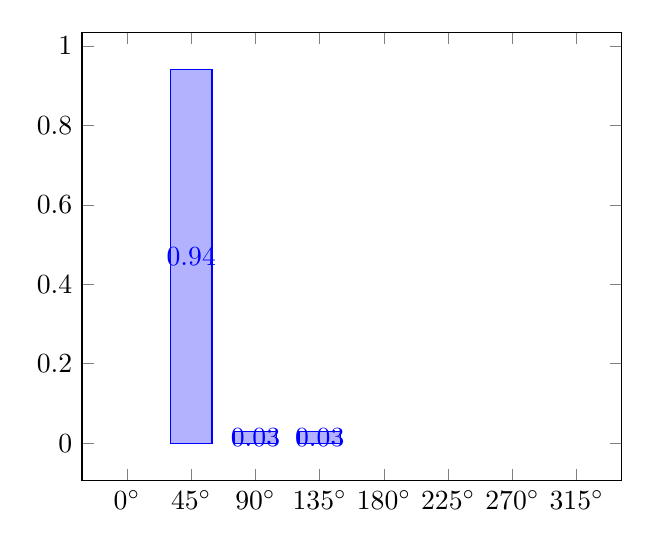
\begin{tikzpicture}
			\begin{axis}[
					ybar stacked,
					bar width=15pt,
					nodes near coords ={\pgfmathprintnumber[fixed] \pgfplotspointmeta},
					symbolic x coords={bin1, bin2, bin3, bin4,
							bin5, bin6, bin7, bin8},
					xtick=data,
					xticklabels={$0^\circ$,
							$45^\circ$,
							$90^\circ$,
							$135^\circ$,
							$180^\circ$,
							$225^\circ$,
							$270^\circ$,
							$315^\circ$,
						}
				]
				\addplot+[ybar] plot coordinates {(bin1,0) (bin2,0.94) (bin3, 0.03) (bin4, 0.03) (bin5,0) (bin6,0) (bin7,0) (bin8,0)};
			\end{axis}
		\end{tikzpicture}
		\caption{Obere Teilregion}
	\end{subfigure}
	\par\bigskip
	\begin{subfigure}{\textwidth}
		\centering
		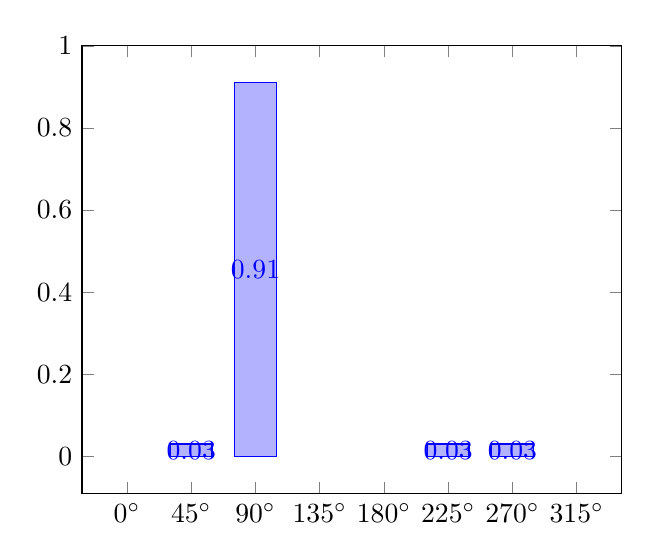
\begin{tikzpicture}
			\begin{axis}[
					ybar stacked,
					bar width=15pt,
					nodes near coords ={\pgfmathprintnumber[fixed] \pgfplotspointmeta},
					symbolic x coords={bin1, bin2, bin3, bin4,
							bin5, bin6, bin7, bin8},
					xtick=data,
					xticklabels={$0^\circ$,
							$45^\circ$,
							$90^\circ$,
							$135^\circ$,
							$180^\circ$,
							$225^\circ$,
							$270^\circ$,
							$315^\circ$,
						},
				]
				\addplot+[ybar] plot coordinates {(bin1,0) (bin2,0.03) (bin3,0.91) (bin4,0) (bin5,0) (bin6,0.03) (bin7,0.03) (bin8,0)};
			\end{axis}
		\end{tikzpicture}
		\caption{Untere Teilregion}
	\end{subfigure}
	\caption{Normalisiertes Orientierungshistogramm}
\end{figure}